% Options for packages loaded elsewhere
\PassOptionsToPackage{unicode}{hyperref}
\PassOptionsToPackage{hyphens}{url}
%
\documentclass[
]{article}
\usepackage{lmodern}
\usepackage{amssymb,amsmath}
\usepackage{ifxetex,ifluatex}
\ifnum 0\ifxetex 1\fi\ifluatex 1\fi=0 % if pdftex
  \usepackage[T1]{fontenc}
  \usepackage[utf8]{inputenc}
  \usepackage{textcomp} % provide euro and other symbols
\else % if luatex or xetex
  \usepackage{unicode-math}
  \defaultfontfeatures{Scale=MatchLowercase}
  \defaultfontfeatures[\rmfamily]{Ligatures=TeX,Scale=1}
\fi
% Use upquote if available, for straight quotes in verbatim environments
\IfFileExists{upquote.sty}{\usepackage{upquote}}{}
\IfFileExists{microtype.sty}{% use microtype if available
  \usepackage[]{microtype}
  \UseMicrotypeSet[protrusion]{basicmath} % disable protrusion for tt fonts
}{}
\makeatletter
\@ifundefined{KOMAClassName}{% if non-KOMA class
  \IfFileExists{parskip.sty}{%
    \usepackage{parskip}
  }{% else
    \setlength{\parindent}{0pt}
    \setlength{\parskip}{6pt plus 2pt minus 1pt}}
}{% if KOMA class
  \KOMAoptions{parskip=half}}
\makeatother
\usepackage{xcolor}
\IfFileExists{xurl.sty}{\usepackage{xurl}}{} % add URL line breaks if available
\IfFileExists{bookmark.sty}{\usepackage{bookmark}}{\usepackage{hyperref}}
\hypersetup{
  pdftitle={Decision Modeling for Publich Health},
  pdfauthor={The DARTH workgroup},
  hidelinks,
  pdfcreator={LaTeX via pandoc}}
\urlstyle{same} % disable monospaced font for URLs
\usepackage[margin=1in]{geometry}
\usepackage{longtable,booktabs}
% Correct order of tables after \paragraph or \subparagraph
\usepackage{etoolbox}
\makeatletter
\patchcmd\longtable{\par}{\if@noskipsec\mbox{}\fi\par}{}{}
\makeatother
% Allow footnotes in longtable head/foot
\IfFileExists{footnotehyper.sty}{\usepackage{footnotehyper}}{\usepackage{footnote}}
\makesavenoteenv{longtable}
\usepackage{graphicx,grffile}
\makeatletter
\def\maxwidth{\ifdim\Gin@nat@width>\linewidth\linewidth\else\Gin@nat@width\fi}
\def\maxheight{\ifdim\Gin@nat@height>\textheight\textheight\else\Gin@nat@height\fi}
\makeatother
% Scale images if necessary, so that they will not overflow the page
% margins by default, and it is still possible to overwrite the defaults
% using explicit options in \includegraphics[width, height, ...]{}
\setkeys{Gin}{width=\maxwidth,height=\maxheight,keepaspectratio}
% Set default figure placement to htbp
\makeatletter
\def\fps@figure{htbp}
\makeatother
\setlength{\emergencystretch}{3em} % prevent overfull lines
\providecommand{\tightlist}{%
  \setlength{\itemsep}{0pt}\setlength{\parskip}{0pt}}
\setcounter{secnumdepth}{-\maxdimen} % remove section numbering

\title{Decision Modeling for Publich Health}
\usepackage{etoolbox}
\makeatletter
\providecommand{\subtitle}[1]{% add subtitle to \maketitle
  \apptocmd{\@title}{\par {\large #1 \par}}{}{}
}
\makeatother
\subtitle{Exercises -- Calibration}
\author{The DARTH workgroup}
\date{}

\begin{document}
\maketitle

Developed by the Decision Analysis in R for Technologies in Health
(DARTH) workgroup:

Fernando Alarid-Escudero, PhD (1)

Eva A. Enns, MS, PhD (2)

M.G. Myriam Hunink, MD, PhD (3,4)

Hawre J. Jalal, MD, PhD (5)

Eline M. Krijkamp, MSc (3)

Petros Pechlivanoglou, PhD (6)

Alan Yang, MSc (7)

In collaboration of:

\begin{enumerate}
\def\labelenumi{\arabic{enumi}.}
\tightlist
\item
  Drug Policy Program, Center for Research and Teaching in Economics
  (CIDE) - CONACyT, Aguascalientes, Mexico
\item
  University of Minnesota School of Public Health, Minneapolis, MN, USA
\item
  Erasmus MC, Rotterdam, The Netherlands
\item
  Harvard T.H. Chan School of Public Health, Boston, USA
\item
  University of Pittsburgh Graduate School of Public Health, Pittsburgh,
  PA, USA
\item
  The Hospital for Sick Children, Toronto and University of Toronto,
  Toronto ON, Canada
\item
  The Hospital for Sick Children, Toronto ON, Canada
\end{enumerate}

Please cite our publications when using this code:

\begin{itemize}
\item
  Jalal H, Pechlivanoglou P, Krijkamp E, Alarid-Escudero F, Enns E,
  Hunink MG. An Overview of R in Health Decision Sciences. Med Decis
  Making. 2017; 37(3): 735-746.
  \url{https://journals.sagepub.com/doi/abs/10.1177/0272989X16686559}
\item
  Krijkamp EM, Alarid-Escudero F, Enns EA, Jalal HJ, Hunink MGM,
  Pechlivanoglou P. Microsimulation modeling for health decision
  sciences using R: A tutorial. Med Decis Making. 2018;38(3):400--22.
  \url{https://journals.sagepub.com/doi/abs/10.1177/0272989X18754513}
\item
  Krijkamp EM, Alarid-Escudero F, Enns E, Pechlivanoglou P, Hunink MM,
  Jalal H. A Multidimensional Array Representation of State-Transition
  Model Dynamics. BioRxiv 670612
  2019.https://www.biorxiv.org/content/10.1101/670612v1
\end{itemize}

Copyright 2017, THE HOSPITAL FOR SICK CHILDREN AND THE COLLABORATING
INSTITUTIONS. All rights reserved in Canada, the United States and
worldwide. Copyright, trademarks, trade names and any and all associated
intellectual property are exclusively owned by THE HOSPITAL FOR Sick
CHILDREN and the collaborating institutions. These materials may be
used, reproduced, modified, distributed and adapted with proper
attribution.

\hypertarget{exercise-calibration-of-a-sick-sicker-model}{%
\section{Exercise: Calibration of a Sick-Sicker
Model}\label{exercise-calibration-of-a-sick-sicker-model}}

In this exercise, we will calibrate a model of a hypothetical
Sick-Sicker disease. A Markov model of the Sick-Sicker disease has been
implemented using four health states: Healthy (H); two disease states,
Sick (S1) and Sicker (S2); and Dead (D). A state transition diagram is
shown in Figure 1. All individuals start in the Healthy state (H). Over
time, healthy individuals may develop the disease and can progress to
S1. Individuals in S1 can recover (return to state H), progress further
to S2 or die. Once in S2, individuals cannot recover (i.e.~cannot
transition back to either S1 or H). Individuals in H have a baseline
probability of death, while individuals in S1 and S2 have an increased
mortality rate compared to healthy individuals, modeled as a hazard
ratio applied to the baseline mortality rate.

Unfortunately, while we can identify those who are afflicted with the
illness through obvious symptoms, we can't easily distinguish those in
the S1 state from the those in the S2 state. Thus, we can't directly
estimate state-specific mortality hazard ratios, nor do we know the
transition probability of progressing from S1 to S2. We do have some
idea of the plausible ranges for these unknown parameters; these ranges
are listed in Table 1. All other model parameters are known and are also
listed in Table 1.

There are three calibration targets to be used in this example: (1)
observed survival of a cohort over time; (2) disease prevalence in a
cohort over time; and (3) among sick patients (S1+S2), the proportion
who are in the S1 state at three points in time. The first two targets
came from an observational study of a typical cohort of individuals. The
third target was obtained by subjecting ill patients to an invasive
procedure which can determine disease stage but can't be used routinely
due to its invasiveness. The calibration target values are provided in
the data file ``SickSicker\_CalibTargets.RData'', which contains a list
with three data frames: Surv, Prev, and PropSick.

\hypertarget{tasks}{%
\subsection{Tasks}\label{tasks}}

\begin{enumerate}
\def\labelenumi{\arabic{enumi}.}
\tightlist
\item
  Use the \texttt{R} script \texttt{SickSicker\_CalibTemplate.R} as a
  starting point to code the calibration of the Sick-Sicker.
\end{enumerate}

\begin{itemize}
\item
  Load and plot the calibration target data stored in
  \texttt{SickSicker\_CalibTargets.RData}.
\item
  Source the file, \texttt{SickSicker\_MarkovModel\_Function.R}, which
  contains the Sick-Sicker model function,
  \texttt{run\_sick\_sicker\_markov()}. This function takes in a vector
  of three parameters, \texttt{c(p\_S1S2,\ hr\_S1,\ hr\_S2)}, and
  returns model outputs corresponding to the calibration targets. Try
  using the model function and look at the output.
\end{itemize}

\begin{enumerate}
\def\labelenumi{\arabic{enumi}.}
\setcounter{enumi}{1}
\tightlist
\item
  Implement the calibration of the Sick-Sicker model using random search
  with 1000 random samples. Copy code from the calibration of the
  3-state model, modifying where necessary. Remember that the
  Sick-Sicker model needs to be calibrated to three different targets
  (instead of one) by varying three different inputs (instead of two).
\end{enumerate}

\begin{itemize}
\item
  Explore the top-fitting input sets (e.g.~top 10, top 100). To
  visualize the best-fitting sets, use \texttt{pairs.panels()} and
  \texttt{scatterplot3d()} functions. Type ``?scatterplot3d'' for
  function documentation.
\item
  Plot the model-predicted output at the best-fitting parameter set
  overlaid over each of the three types of calibration targets (extend
  the plotting code in the 3-state model calibration script).
\end{itemize}

\begin{enumerate}
\def\labelenumi{\arabic{enumi}.}
\setcounter{enumi}{2}
\tightlist
\item
  Save a new copy of your Sick-Sicker model calibration code. Change the
  implementation from random search to Nelder-Mead, using 100 random
  starting points. Where do you need to make changes? Use the
  Nelder-Mead calibration of the 3-state model as a guide.
\end{enumerate}

\begin{itemize}
\item
  Explore the top-fitting input sets (e.g.~top 10) using
  \texttt{pairs.panels()} and \texttt{scatterplot3d()}. How does it
  compare to the best-fitting sets from random search?
\item
  Plot the model-predicted output at the best-fitting parameter set
  overlaid over each of the three types of calibration targets.
\end{itemize}

\begin{enumerate}
\def\labelenumi{\arabic{enumi}.}
\setcounter{enumi}{3}
\tightlist
\item
  Save a new copy of your Sick-Sicker model calibration code. Use the
  Bayesian calibration of the 3-state model as a guide and modify your
  Sick-Sicker calibration code to implement the IMIS calibration method.
\end{enumerate}

\begin{itemize}
\item
  Sample 1,000 parameter sets from the calibrated posterior
  distribution. Visualize these parameter sets using
  \texttt{scatterplot3d()} and \texttt{pairs.panels()}.
\item
  Plot the model-predicted output at the maximum aposteriori parameter
  set overlaid over each of the three types of calibration targets.
\end{itemize}

\textbf{Table 1: Input parameters for the time dependent Sick-Sicker
Microsimulation }

\begin{longtable}[]{@{}llc@{}}
\toprule
\begin{minipage}[b]{0.51\columnwidth}\raggedright
\textbf{Parameter}\strut
\end{minipage} & \begin{minipage}[b]{0.19\columnwidth}\raggedright
\textbf{R name}\strut
\end{minipage} & \begin{minipage}[b]{0.21\columnwidth}\centering
\textbf{Value}\strut
\end{minipage}\tabularnewline
\midrule
\endhead
\begin{minipage}[t]{0.51\columnwidth}\raggedright
Time horizon\strut
\end{minipage} & \begin{minipage}[t]{0.19\columnwidth}\raggedright
\texttt{n\_t}\strut
\end{minipage} & \begin{minipage}[t]{0.21\columnwidth}\centering
30 years\strut
\end{minipage}\tabularnewline
\begin{minipage}[t]{0.51\columnwidth}\raggedright
Cycle length\strut
\end{minipage} & \begin{minipage}[t]{0.19\columnwidth}\raggedright
\strut
\end{minipage} & \begin{minipage}[t]{0.21\columnwidth}\centering
1 year\strut
\end{minipage}\tabularnewline
\begin{minipage}[t]{0.51\columnwidth}\raggedright
Names of simulated individuals\strut
\end{minipage} & \begin{minipage}[t]{0.19\columnwidth}\raggedright
\texttt{n\_i}\strut
\end{minipage} & \begin{minipage}[t]{0.21\columnwidth}\centering
1000\strut
\end{minipage}\tabularnewline
\begin{minipage}[t]{0.51\columnwidth}\raggedright
Names of health states\strut
\end{minipage} & \begin{minipage}[t]{0.19\columnwidth}\raggedright
\texttt{v\_n}\strut
\end{minipage} & \begin{minipage}[t]{0.21\columnwidth}\centering
H, S1, S2, D\strut
\end{minipage}\tabularnewline
\begin{minipage}[t]{0.51\columnwidth}\raggedright
Annual discount rate (costs/QALYs)\strut
\end{minipage} & \begin{minipage}[t]{0.19\columnwidth}\raggedright
\texttt{d\_r}\strut
\end{minipage} & \begin{minipage}[t]{0.21\columnwidth}\centering
3\%\strut
\end{minipage}\tabularnewline
\begin{minipage}[t]{0.51\columnwidth}\raggedright
Annual transition probabilities\strut
\end{minipage} & \begin{minipage}[t]{0.19\columnwidth}\raggedright
\strut
\end{minipage} & \begin{minipage}[t]{0.21\columnwidth}\centering
\strut
\end{minipage}\tabularnewline
\begin{minipage}[t]{0.51\columnwidth}\raggedright
- Disease onset (H to S1)\strut
\end{minipage} & \begin{minipage}[t]{0.19\columnwidth}\raggedright
\texttt{p\_HS1}\strut
\end{minipage} & \begin{minipage}[t]{0.21\columnwidth}\centering
0.15\strut
\end{minipage}\tabularnewline
\begin{minipage}[t]{0.51\columnwidth}\raggedright
- Recovery (S1 to H)\strut
\end{minipage} & \begin{minipage}[t]{0.19\columnwidth}\raggedright
\texttt{p\_S1H}\strut
\end{minipage} & \begin{minipage}[t]{0.21\columnwidth}\centering
0.5\strut
\end{minipage}\tabularnewline
\begin{minipage}[t]{0.51\columnwidth}\raggedright
- Disease progression (S1 to S2)\strut
\end{minipage} & \begin{minipage}[t]{0.19\columnwidth}\raggedright
\texttt{p\_S1S2}\strut
\end{minipage} & \begin{minipage}[t]{0.21\columnwidth}\centering
To be calibrated; range: 0.01 - 0.50\strut
\end{minipage}\tabularnewline
\begin{minipage}[t]{0.51\columnwidth}\raggedright
Annual mortality\strut
\end{minipage} & \begin{minipage}[t]{0.19\columnwidth}\raggedright
\strut
\end{minipage} & \begin{minipage}[t]{0.21\columnwidth}\centering
\strut
\end{minipage}\tabularnewline
\begin{minipage}[t]{0.51\columnwidth}\raggedright
- All-cause mortality (H to D)\strut
\end{minipage} & \begin{minipage}[t]{0.19\columnwidth}\raggedright
\texttt{p\_HD}\strut
\end{minipage} & \begin{minipage}[t]{0.21\columnwidth}\centering
0.005\strut
\end{minipage}\tabularnewline
\begin{minipage}[t]{0.51\columnwidth}\raggedright
- Hazard ratio of death in S1 vs H\strut
\end{minipage} & \begin{minipage}[t]{0.19\columnwidth}\raggedright
\texttt{hr\_S1}\strut
\end{minipage} & \begin{minipage}[t]{0.21\columnwidth}\centering
To be calibrated; range: 1.0 - 4.5\strut
\end{minipage}\tabularnewline
\begin{minipage}[t]{0.51\columnwidth}\raggedright
- Hazard ratio of death in S2 vs H\strut
\end{minipage} & \begin{minipage}[t]{0.19\columnwidth}\raggedright
\texttt{hr\_S2}\strut
\end{minipage} & \begin{minipage}[t]{0.21\columnwidth}\centering
To be calibrated; range: 5 - 15\strut
\end{minipage}\tabularnewline
\begin{minipage}[t]{0.51\columnwidth}\raggedright
Annual costs\strut
\end{minipage} & \begin{minipage}[t]{0.19\columnwidth}\raggedright
\strut
\end{minipage} & \begin{minipage}[t]{0.21\columnwidth}\centering
\strut
\end{minipage}\tabularnewline
\begin{minipage}[t]{0.51\columnwidth}\raggedright
- Healthy individuals\strut
\end{minipage} & \begin{minipage}[t]{0.19\columnwidth}\raggedright
\texttt{c\_H}\strut
\end{minipage} & \begin{minipage}[t]{0.21\columnwidth}\centering
\$2,000\strut
\end{minipage}\tabularnewline
\begin{minipage}[t]{0.51\columnwidth}\raggedright
- Sick individuals in S1\strut
\end{minipage} & \begin{minipage}[t]{0.19\columnwidth}\raggedright
\texttt{c\_S1}\strut
\end{minipage} & \begin{minipage}[t]{0.21\columnwidth}\centering
\$4,000\strut
\end{minipage}\tabularnewline
\begin{minipage}[t]{0.51\columnwidth}\raggedright
- Sick individuals in S2\strut
\end{minipage} & \begin{minipage}[t]{0.19\columnwidth}\raggedright
\texttt{c\_S2}\strut
\end{minipage} & \begin{minipage}[t]{0.21\columnwidth}\centering
\$15,000\strut
\end{minipage}\tabularnewline
\begin{minipage}[t]{0.51\columnwidth}\raggedright
- Dead individuals\strut
\end{minipage} & \begin{minipage}[t]{0.19\columnwidth}\raggedright
\texttt{c\_D}\strut
\end{minipage} & \begin{minipage}[t]{0.21\columnwidth}\centering
\$0\strut
\end{minipage}\tabularnewline
\begin{minipage}[t]{0.51\columnwidth}\raggedright
- Additional costs of sick individuals treated in S1 or S2\strut
\end{minipage} & \begin{minipage}[t]{0.19\columnwidth}\raggedright
\texttt{c\_trt}\strut
\end{minipage} & \begin{minipage}[t]{0.21\columnwidth}\centering
\$12,000\strut
\end{minipage}\tabularnewline
\begin{minipage}[t]{0.51\columnwidth}\raggedright
Utility weights\strut
\end{minipage} & \begin{minipage}[t]{0.19\columnwidth}\raggedright
\strut
\end{minipage} & \begin{minipage}[t]{0.21\columnwidth}\centering
\strut
\end{minipage}\tabularnewline
\begin{minipage}[t]{0.51\columnwidth}\raggedright
- Healthy individuals\strut
\end{minipage} & \begin{minipage}[t]{0.19\columnwidth}\raggedright
\texttt{u\_H}\strut
\end{minipage} & \begin{minipage}[t]{0.21\columnwidth}\centering
1.00\strut
\end{minipage}\tabularnewline
\begin{minipage}[t]{0.51\columnwidth}\raggedright
- Sick individuals in S1\strut
\end{minipage} & \begin{minipage}[t]{0.19\columnwidth}\raggedright
\texttt{u\_S1}\strut
\end{minipage} & \begin{minipage}[t]{0.21\columnwidth}\centering
0.75\strut
\end{minipage}\tabularnewline
\begin{minipage}[t]{0.51\columnwidth}\raggedright
- Sick individuals in S2\strut
\end{minipage} & \begin{minipage}[t]{0.19\columnwidth}\raggedright
\texttt{u\_S2}\strut
\end{minipage} & \begin{minipage}[t]{0.21\columnwidth}\centering
0.50\strut
\end{minipage}\tabularnewline
\begin{minipage}[t]{0.51\columnwidth}\raggedright
- Dead individuals\strut
\end{minipage} & \begin{minipage}[t]{0.19\columnwidth}\raggedright
\texttt{u\_D}\strut
\end{minipage} & \begin{minipage}[t]{0.21\columnwidth}\centering
0.00\strut
\end{minipage}\tabularnewline
\begin{minipage}[t]{0.51\columnwidth}\raggedright
Intervention effect\strut
\end{minipage} & \begin{minipage}[t]{0.19\columnwidth}\raggedright
\strut
\end{minipage} & \begin{minipage}[t]{0.21\columnwidth}\centering
\strut
\end{minipage}\tabularnewline
\begin{minipage}[t]{0.51\columnwidth}\raggedright
- Utility for treated individuals in S1\strut
\end{minipage} & \begin{minipage}[t]{0.19\columnwidth}\raggedright
\texttt{u\_trt}\strut
\end{minipage} & \begin{minipage}[t]{0.21\columnwidth}\centering
0.95\strut
\end{minipage}\tabularnewline
\bottomrule
\end{longtable}

\begin{figure}

{\centering 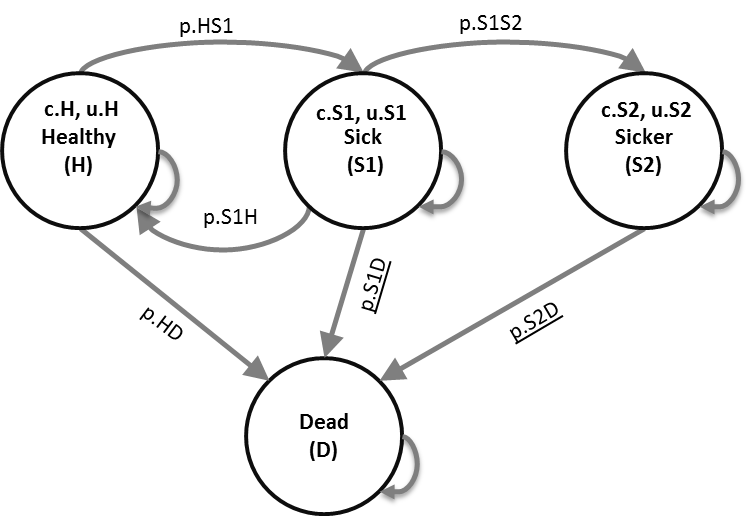
\includegraphics[width=1\linewidth]{sick_sicker_diagram} 

}

\caption{Schematic representation of the Sick-Sicker model}\label{fig:unnamed-chunk-1}
\end{figure}

\end{document}
